% !TEX root = main.tex

\section{Experiments}
In this section, we conduct experiments to evaluate the performance of our method via node classification on ETG.

\subsection{Data Collection and Graph Construction}
We collect all data by running Ethereum client\footnote{Parity Ethereum Client, https://www.parity.io/ethereum/} which maintains the same copy of blockchain with all historical transactions. Note that we choose the transaction logs on Ethereum from January 1, 2018 to March 31, 2018 (\textcolor{red}{xxxx} external transactions and internal transactions both) as the input of graph construction since it is the most active period with various activities.

By parsing the transactions, 16,599,825 active accounts are obtained, including 14,450,993 EOAs and 2,148,831 SCs (the remaining address is \textcolor{red}{0x000}). Then we construct the original ETG based on these accounts and transactions.

\begin{figure}[htbp]
\centering
\begin{tabular}{cc}
	\subfigure[Histogram of time std for all nodes.]{
		\label{fig:high_order}
		%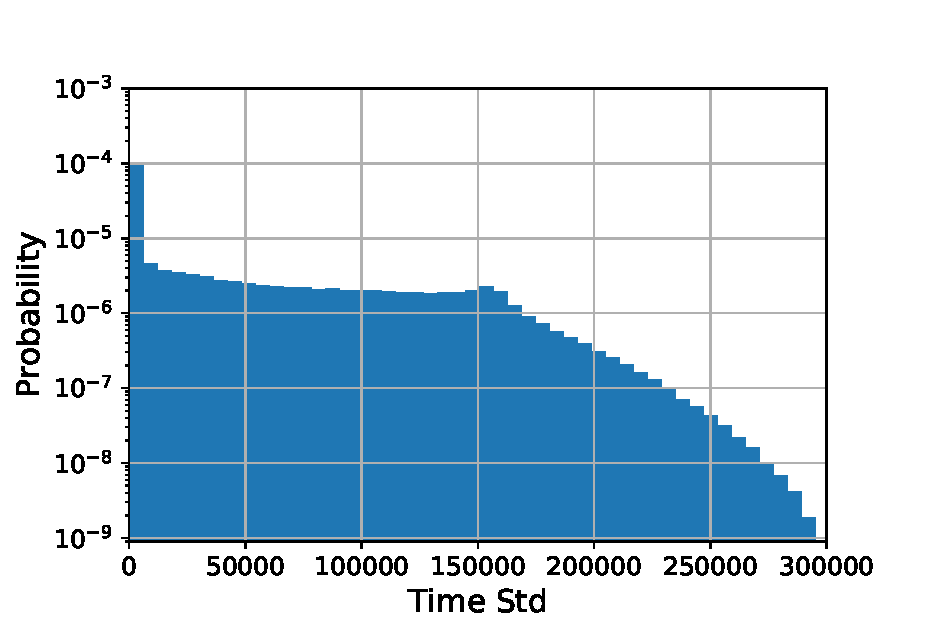
\includegraphics[width=0.22\textwidth]{fig/all_time_std_pdf.eps}
    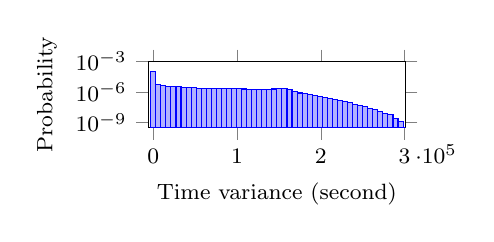
\begin{tikzpicture}
\begin{axis}[ymax=0.001,ybar,ymode=log,bar width=6023.807139652907,log origin=infty,xmin=-6023.807139652907,ytick align=outside,enlargelimits=0,
width=.40\textwidth,
height=.20\textwidth,
ylabel=Probability,
xlabel=Time variance (second),
every x tick scale label/.style={at={(xticklabel cs:1)},anchor=south west},
  label style={font=\footnotesize},
tick label style={font=\footnotesize} ,
]
\addplot  plot coordinates {
(0.0, 9.451382865223466e-05)
(6023.807139652907, 5.4237855234498505e-06)
(12047.614279305813, 4.160561994558263e-06)
(18071.421418958722, 3.567714777734051e-06)
(24095.228558611627, 3.385128656276782e-06)
(30119.03569826453, 3.165308635083816e-06)
(36142.842837917444, 2.9615307529739165e-06)
(42166.64997757035, 2.6626153921894407e-06)
(48190.45711722325, 2.5490152149843527e-06)
(54214.26425687616, 2.3890921746281617e-06)
(60238.07139652906, 2.275444535473124e-06)
(66261.87853618198, 2.248248838151831e-06)
(72285.68567583489, 2.156718467673447e-06)
(78309.49281548779, 2.138350693042835e-06)
(84333.2999551407, 2.0591366985764506e-06)
(90357.1070947936, 2.0862137410228693e-06)
(96380.9142344465, 2.0135969575995206e-06)
(102404.72137409942, 2.000948347937872e-06)
(108428.52851375232, 1.9544830989369192e-06)
(114452.33565340523, 1.9188391745245435e-06)
(120476.14279305813, 1.8834088288869425e-06)
(126499.94993271104, 1.8642104701322076e-06)
(132523.75707236395, 1.8633324240581345e-06)
(138547.56421201685, 1.8347365992133192e-06)
(144571.37135166978, 1.9392715439779758e-06)
(150595.17849132267, 2.1352419353211166e-06)
(156618.98563097557, 2.1487685910568386e-06)
(162642.79277062847, 1.6649889352174985e-06)
(168666.5999102814, 1.0367825656806102e-06)
(174690.4070499343, 7.939434987619423e-07)
(180714.2141895872, 6.496829018892185e-07)
(186738.02132924012, 5.151757357311993e-07)
(192761.828468893, 4.3131047016972446e-07)
(198785.6356085459, 3.5105231280444205e-07)
(204809.44274819884, 2.852225882239295e-07)
(210833.24988785174, 2.272003544101756e-07)
(216857.05702750463, 1.7961974958539996e-07)
(222880.86416715756, 1.4827113164349042e-07)
(228904.67130681046, 1.1445449230418602e-07)
(234928.47844646336, 8.545524088479658e-08)
(240952.28558611625, 6.371766780774196e-08)
(246976.09272576918, 4.777045262457526e-08)
(252999.89986542208, 3.780344313509607e-08)
(259023.70700507498, 2.6009148572545693e-08)
(265047.5141447279, 1.8557622430411254e-08)
(271071.3212843808, 1.31232291611476e-08)
(277095.1284240337, 8.305841241232658e-09)
(283118.9355636866, 5.624241069063257e-09)
(289142.74270333955, 2.7053311471443514e-09)
(295166.54984299245, 1.3526655735721757e-09)
(301190.35698264535, 3.0850267467435584e-10)
};\end{axis}
\end{tikzpicture}

	%\caption{Example of a high-order proximity caption.}
	}&
	\subfigure[Histogram of time std for hack\&phish nodes.]{
		\label{fig:asymmetric}
		%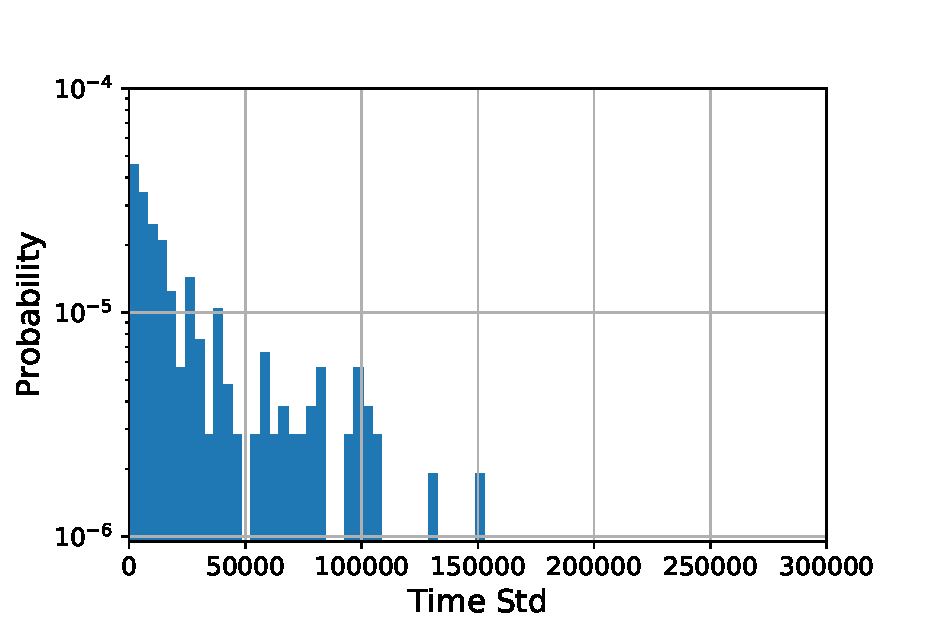
\includegraphics[width=0.22\textwidth]{fig/fake_time_std_pdf.eps}
    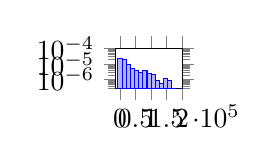
\begin{tikzpicture}
\begin{axis}[ymax=0.0001,ybar,ymode=log,bar width=13410.783587930588,log origin=infty,xmin=-13410.783587930588,ytick align=outside,enlargelimits=0,
width=.20\textwidth,
every x tick scale label/.style={at={(xticklabel cs:1)},anchor=south west},
]
\addplot  plot coordinates {
(0.0, 2.1630081044550223e-05)
(13410.783587930588, 1.9637836737815332e-05)
(26821.567175861175, 8.822796215540222e-06)
(40232.350763791765, 5.122913931604e-06)
(53643.13435172235, 3.699882283936222e-06)
(67053.91793965294, 2.8460632953355556e-06)
(80464.70152758353, 3.984488613469778e-06)
(93875.48511551411, 2.561456965802e-06)
(107286.2687034447, 2.2768506362684445e-06)
(120697.0522913753, 8.538189886006666e-07)
(134107.83587930587, 5.692126590671111e-07)
(147518.61946723645, 1.1384253181342222e-06)
(160929.40305516706, 8.538189886006666e-07)
(174340.18664309764, 2.8460632953355556e-07)
(187750.97023102822, 0.0)
(201161.75381895882, 2.8460632953355556e-07)
};\end{axis}
\end{tikzpicture}

	}
\end{tabular}
\caption{Examples.}
\end{figure}

Specially, we extend the pre-processing scheme to adapt our model. First we construct four relation graphs, which contains ETH transfer graph, contract creation graph, contract invocation graph and mining reward graph. In each graph, repeated edges between the same node pair are merged via the method introduced in section \ref{section:time}.

Last, a test set of accounts with label introduced before is provided to evaluate classification accuracy. It is hard to reveal the identity of addresses since the anonymity of blockchain. We obtain these labeled examples in two ways, \emph{Etherscan}\footnote{Etherscan LabelCloud, https://etherscan.io/labelcloud} and \emph{Searchain}\footnote{Searchain, http://www.searchain.io/}.




\subsection{Experimental Set-Up and Baselines}
Unless otherwise noted,

As a baseline for our experiments, we compare against state-of-the-art classification accuracy from \textcolor{red}{XXX, XXX, XXX and XXX}.
\begin{table*}
\footnotesize
\centering
\caption{}
\resizebox{\textwidth}{17mm}{
\begin{tabular}{l|ccc|ccc|ccc|ccc|ccc}
\toprule
& \multicolumn{3}{c|}{Deepwalk} & \multicolumn{3}{c|}{GCN} & \multicolumn{3}{c|}{rGCN} & \multicolumn{3}{c|}{rGCN+asymmetric proximity} & \multicolumn{3}{c|}{Ours} \\
\midrule
& \textbf{Precision} & \textbf{Recall} & $\mathbf{F_1}$ & \textbf{Precision} & \textbf{Recall} & $\mathbf{F_1}$ & \textbf{Precision} & \textbf{Recall} & $\mathbf{F_1}$ & \textbf{Precision} & \textbf{Recall} & $\mathbf{F_1}$ & \textbf{Precision} & \textbf{Recall} & $\mathbf{F_1}$ \\
\midrule
 phish and hack & & & &0.614 & 0.273 & 0.378 & 0.700& 0.778& 0.737& 0.720& 0.727& 0.724& 0.714& 0.758& 0.735\\
 token contract & & & &0.634& 0.459& 0.533& 0.930& 0.949& 0.939& 0.958& 0.939& 0.949& 0.958& 0.939& 0.949\\
 exchange deposit & & & &0.526& 0.400& 0.455& 0.500& 0.280& 0.359& 0.615& 0.640& 0.628& 0.556& 0.600& 0.579\\
 exchange root & & & &0.579& 0.743& 0.650& 0.913& 0.600& 0.724& 0.862& 0.714& 0.781& 0.828& 0.686& 0.750\\
 pool & & & &0.344& 0.500& 0.407& 1.000& 0.636& 0.778& 0.842& 0.727& 0.781& 1.000& 0.727& 0.842\\
 miner & & & &0.696& 0.390& 0.500& 0.905& 0.927& 0.916& 0.826& 0.927& 0.874& 0.841& 0.902& 0.871\\
 primary market & & & & 0.238& 0.161& 0.192& 0.786& 0.355& 0.489& 0.680& 0.548& 0.607& 0.750& 0.484& 0.588\\
 ICO wallet & & & & 0.539& 0.184& 0.275& 0.677& 0.552& 0.609& 0.769& 0.526& 0.625& 0.742& 0.605& 0.668\\
 \midrule
 average & & & & 0.566& 0.378& 0.436& 0.807& 0.725& 0.751& 0.806& 0.761& 0.779& \bf{0.811}& \bf{0.764}& \bf{0.782}\\
\bottomrule
\end{tabular}
}
\end{table*}

% \begin{table}
% \centering
% \caption{}
% \begin{tabular}{l|ccc}
% \toprule
% \textbf{Model} & \textbf{Precision}  & \textbf{Recall} & $\mathbf{F_1}$  \\
% \midrule
%  Deepwalk & & & \\
%  GCN & & & \\
%  rGCN & & & \\
%  Our & & & \\
% \midrule
%  w/o time-density& & & \\
%  w/o asymmetric proximity & & & \\
% \bottomrule
% \end{tabular}
% \end{table}

All embedding and classification programs were run on the server, which includes Intel Xeon E5 CPU with 55 processors and 128GB of memory, and the GPU used for deep learning is Nvidia 1080Ti.

\subsection{Results}


%These data are collected

%%% Local Variables:
%%% mode: latex
%%% TeX-master: "analysis"
%%% End:
